\documentclass[20pt,margin=5mm, innermargin=6mm, blockverticalspace=6mm, colspace=6mm]{tikzposter}
\usepackage[utf8]{inputenc}
\geometry{paperwidth=42.0cm,paperheight=59.4cm}
% \usetheme{Simple}
% \usecolorstyle{Spain}
% \usebackgroundstyle{Empty}
% \usetitlestyle{Filled}
% \useblockstyle{Basic}
\tikzposterlatexaffectionproofoff
\usepackage{amsmath}
\usepackage{enumitem}


\useblockstyle[titleinnersep=4mm, bodyverticalshift = -6mm]{Slide}
\renewcommand*\familydefault{cabin}
\usepackage[sfdefault,condensed]{cabin}
\usepackage[T1]{fontenc}
\usepackage{fix-cm}
\usepackage{tikz,multicol}
\usepackage{capt-of}

\definecolor{greenone}{RGB}{21,75,52}
\definecolor{greentwo}{RGB}{25,97,66}
\definecolor{greenthree}{RGB}{16,57,39}
\definecolor{mygray}{RGB}{203,203,203}
\definecolorstyle{myColorStyle} {
    \colorlet{colorOne}{greenone}
    \colorlet{colorTwo}{greentwo}
    \colorlet{colorThree}{greenthree}
    \colorlet{colorFour}{mygray}
    }{
    % Background Colors
    \colorlet{backgroundcolor}{colorOne}
    \colorlet{framecolor}{colorOne}
    % Title Colors
    \colorlet{titlefgcolor}{white}
    \colorlet{titlebgcolor}{colorTwo}
    % Block Colors
    \colorlet{blocktitlebgcolor}{colorFour}
    \colorlet{blocktitlefgcolor}{colorTwo}
    \colorlet{blockbodybgcolor}{white}
    \colorlet{blockbodyfgcolor}{black}
    % Innerblock Colors
    \colorlet{innerblocktitlebgcolor}{white}
    \colorlet{innerblocktitlefgcolor}{black}
    \colorlet{innerblockbodybgcolor}{white}
    \colorlet{innerblockbodyfgcolor}{black}
    % Note colors
    \colorlet{notefgcolor}{black}
    \colorlet{notebgcolor}{white}
    \colorlet{notefrcolor}{white}
}

\usecolorstyle{myColorStyle}

\usebackgroundstyle{Rays}
\usepackage{adjustbox}
\usetitlestyle{Empty}

\makeatletter %To make columns scale to custom width 
\setlength{\TP@visibletextwidth}{\textwidth-2\TP@innermargin}
\setlength{\TP@visibletextheight}{\textheight-2\TP@innermargin}
\makeatother


%shifts bullets to left margin for all document
%\setitemize{itemsep=10pt,topsep=0pt,parsep=0pt,partopsep=0pt, leftmargin=*}

%only for a list
%\begin{itemize}[noitemsep,topsep=0pt,parsep=0pt,partopsep=0pt]
 
%\graphicspath{{images/}}

%%%%%%%%%%%%%%%%%%%%%%%%%%%%%%%%%%%%%%%%%%%%%%%%%%%%%%%%%%%%%%%%%%%%%%%%

\title{\parbox{\linewidth}{\vspace{-4.5cm} \centering \huge Title thinking in process}}
\author{\vspace{-100pt} % space between title and author
  {\begin{minipage}{7.5cm}
    \hfill
    \vspace{-20pt}
    \flushleft
    
\includegraphics[trim=0cm 8cm 0cm 8cm,clip,width=7.5cm]{Imperial_Whitelogo.pdf}
  \end{minipage}
    \vspace{-20pt}
    \hspace{2pt}}
  {\begin{minipage}{22cm}
    \centering
        { \Large Jia Le, Lim \\ \vspace{-20pt}
          \normalsize Department of Life Sciences, Silwood Park Campus, Imperial College London}
  \end{minipage}
    \vspace{-20pt}
  \hspace{2pt}}
  {\begin{minipage}{9cm}
    \hfill
    \flushright
    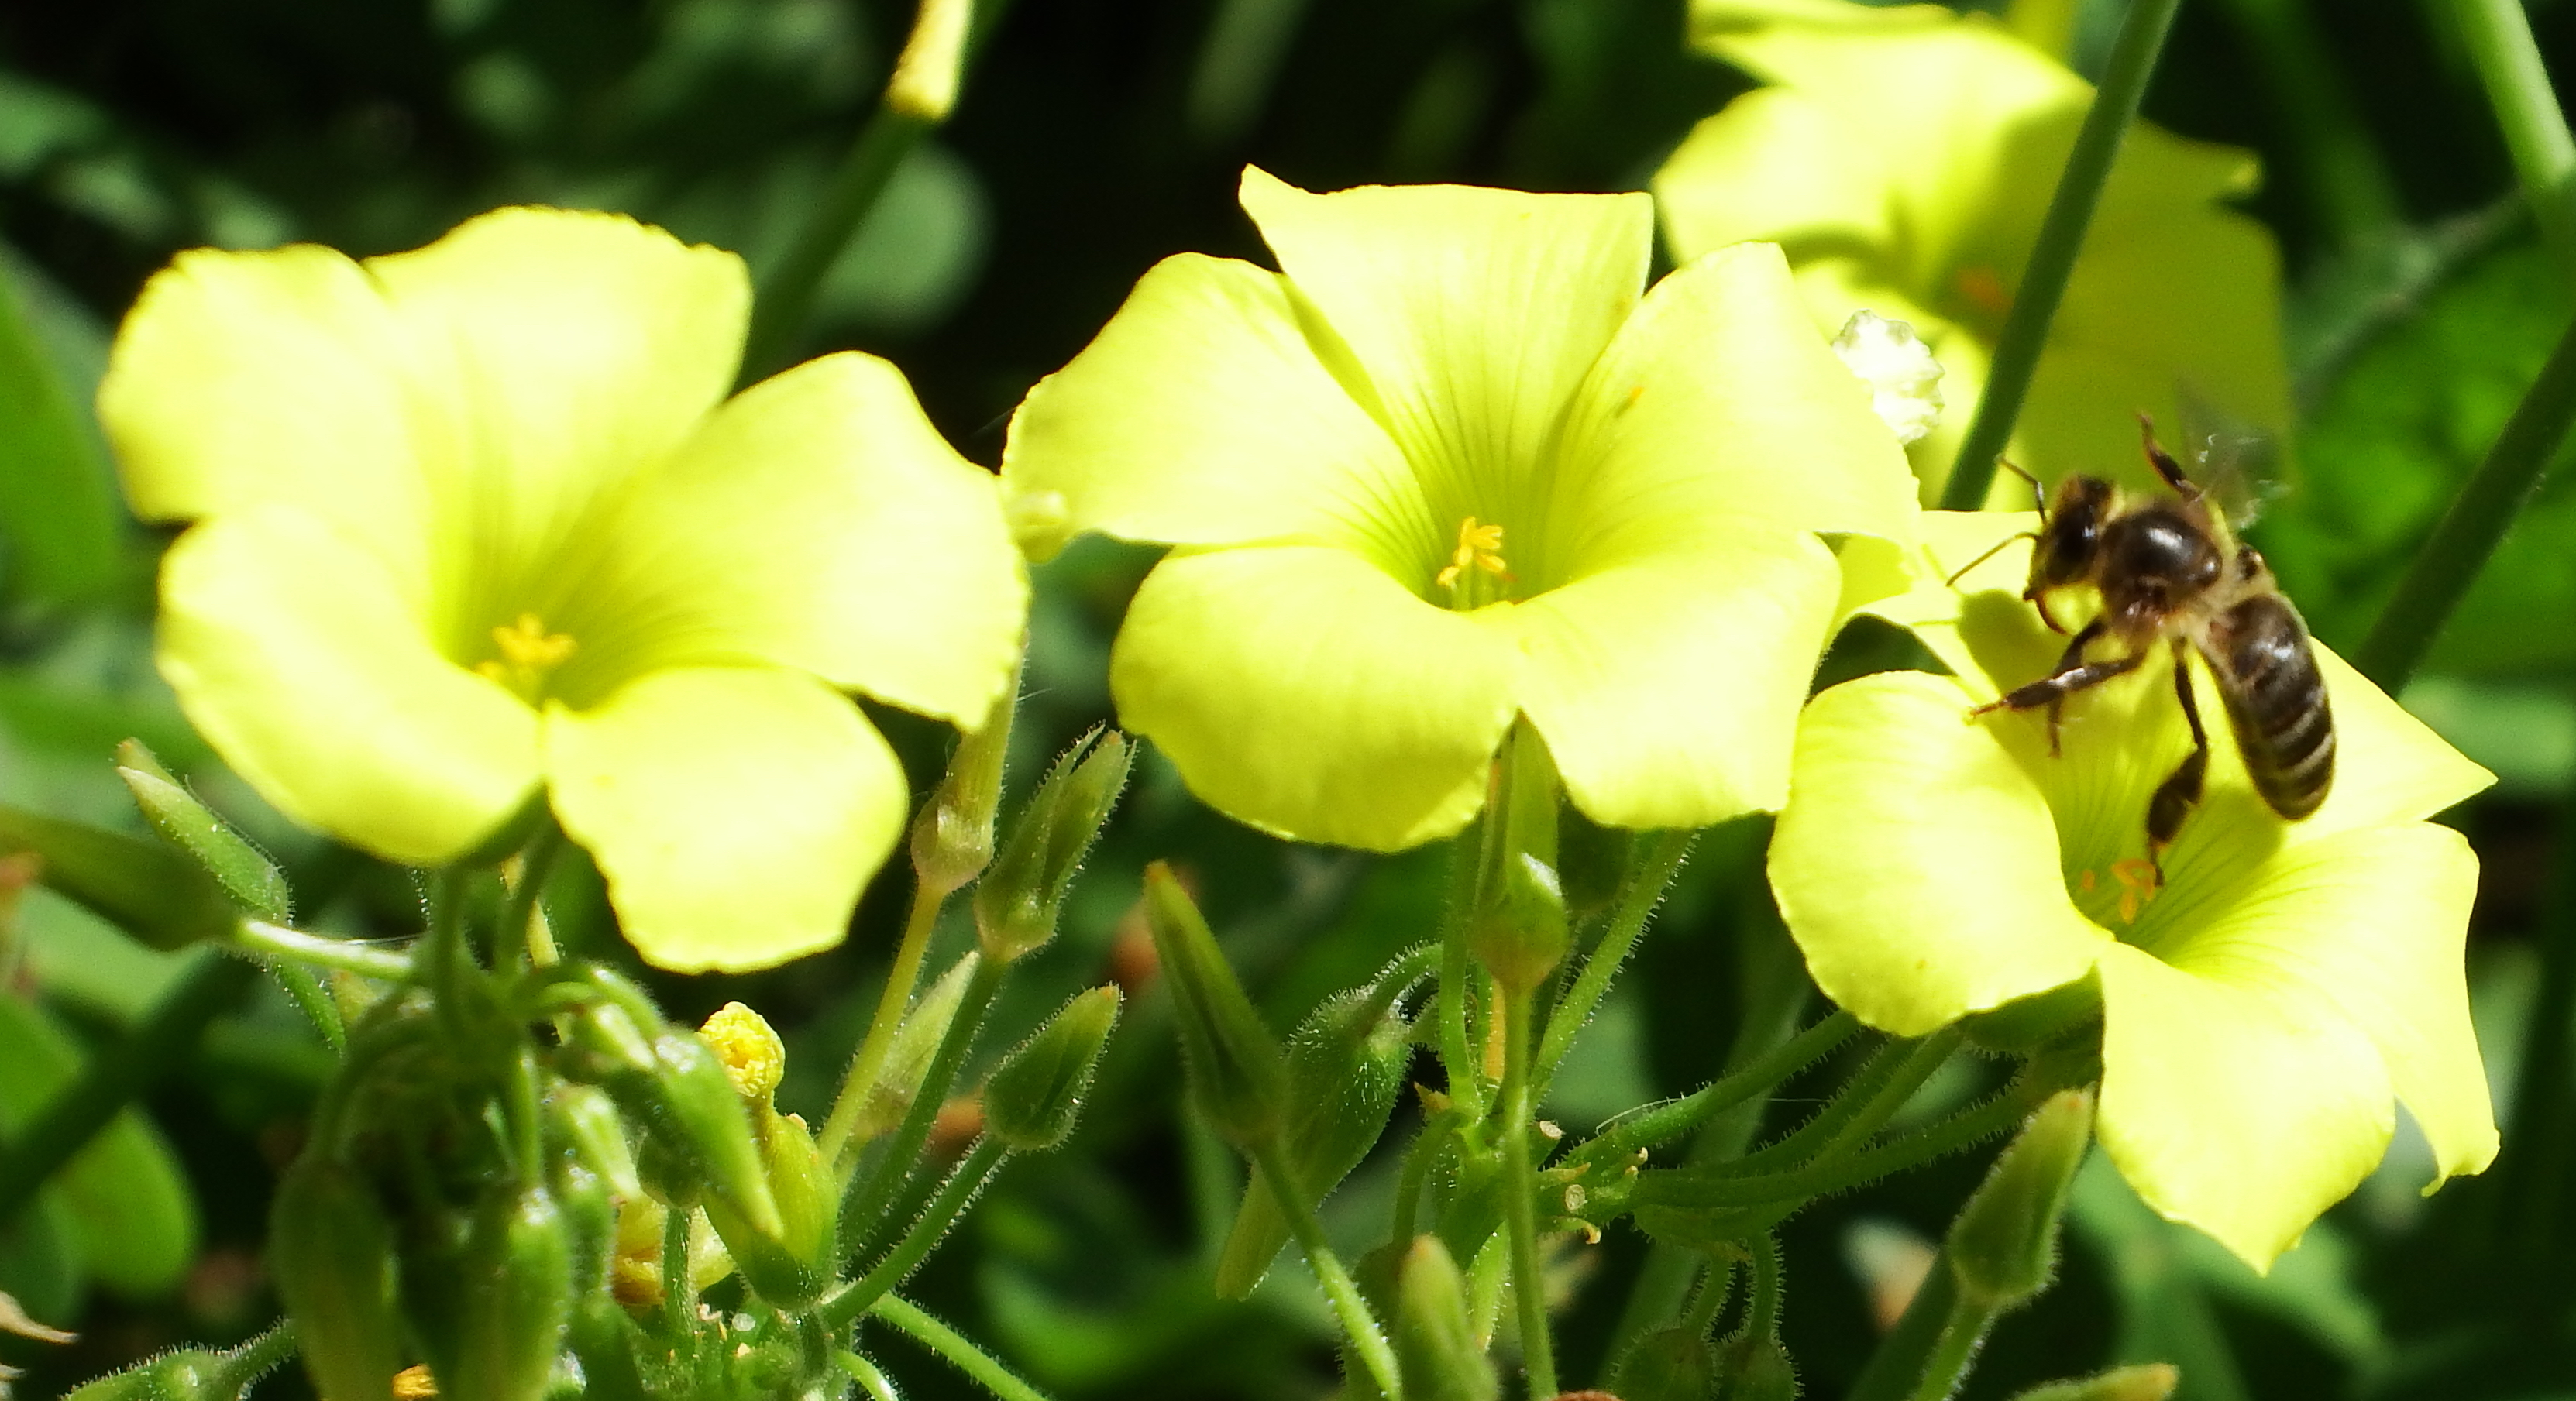
\includegraphics[trim=0cm 8cm 0cm 8cm,clip,width=9cm]{picture.JPG}
  \end{minipage}
  \vspace{-20pt}}
  }

%%%%%%%%%%%%%%%%%%%%%%%%%%%%%%%%%%%%%%%%%%%%%%%%%%%%%%%%%%%%%%%%%%%%%%%%
\makeatletter
\newcommand\semiHUGE{\@setfontsize\semiHUGE{60}{27.38}}
\makeatother

\begin{document}
\node[xshift=-20cm, at=(topright),opacity=0.9]{\includegraphics[width=\paperwidth, height=10cm]{head1low.jpg}} ;

\maketitle[titletoblockverticalspace=2mm]

  %%%%%%%%%%%%%%%%%%%%%%%%%%%%%%%%%%%%%%%%%%%%%%%%%%%%%%%%%%%%%%%%%%%%%%%%
%Introduction in form of a question?
\block{\Large \hspace{11pt} Do bee-flower interactions change over time? }{

  \normalsize
     %Brief Introduction explaining broader significance of research problem and the gap in knowledge that is being addressed
     Previous studies assume that the temperature dependence of ecosystem function is a simple scaling up of all the component species’ thermal responses. In this case, predicting the effects of climatic warming or cooling on ecosystem function would be a relatively straightforward task.  

  \begin{minipage}[]{0.45\linewidth}

   \vspace{15pt}
   \subsection*{Data}
   %Materials and methods

    We combine new theory and data on the temperature dependence of key metabolic traits at both:
    \begin{itemize} \itemsep5pt 
    \item \textit {Species level:} more than 300 different species of terrestrial plants (\textit {Biotraits Database})
    \item \textit{Ecosystem level:} 118 local terrestrial ecosystems across the world (\textit{Fluxnet Database})
    \end {itemize}

  \end{minipage}   
  \hspace{.8cm}    
  \begin{minipage}[]{0.52\linewidth}
 
    \vspace{15pt}
    \subsection*{We ask...}
     %research plan
    \begin{itemize} \itemsep5pt 
    \item Are differences in species-level temperature-dependence of photosynthesis and respiration reflected in the ecosystem thermal response? 
    \item Do the full unimodal thermal responses of metabolic rate matter for mapping individual TPCs to ecosystem-level fluxes?
    \end{itemize}
    
    \end{minipage}
    
    \vspace{15pt}
   %A clear statement of the project aim or aims
We present a preliminary analysis of instraspecific data, to get the patterns necessary for parameterizing a model, and ecosystem flux data for validation.
   
 }

 %%%%%%%%%%%%%%%%%%%%%%%%%%%%%%%%%%%%%%%%%%%%%%%%%%%%%%%%%%%%%%%%%%%%%%%%

\begin{columns}

  \column{0.3}
  \block{\Large \hspace{17pt}Calculating Whittaker's \\ \hspace{17pt}dissimilarity index}{
    \normalsize
A simple equation to map individual metabolism to ecosystem flux on a daily scale is:    
	\vspace{-60pt} \\
	
    \begin{align*}
      F & = F_{0} \Big(\sum_{i=1}^{k} {x_i }
    \end{align*}\\

    \vspace{-40pt}
    where:    
    \begin{itemize}\itemsep15pt
     \item $k$ is an autotroph and $j$ is a heterotroph species 
    \item $\sum_{i=1}^{k} x_i$ is the total biomass of the ecosystem 

    \end{itemize}
    \vspace{-10pt}
    
    A general form for the distribution of biomasses across species is:
    \begin{align*}
      x_i = h(m_i)
    \end{align*}

    that is, $x_{i}$ is a function $h$ of the body mass of the species.  

  }

%%%%%%%%%%%%%%%%%%%%%%%%%%%%%%%%%%%%%%%%%%%%%%%%%%%%%%%%%%%%%%%%%%%%%%%%%%%%%%%%%%%%%%%%%%%%%%%%%%%%%%%%%%%%%%%%%%


  \column{0.7}
  \block{\Large \hspace{17pt} Results}{ 
    \centering
    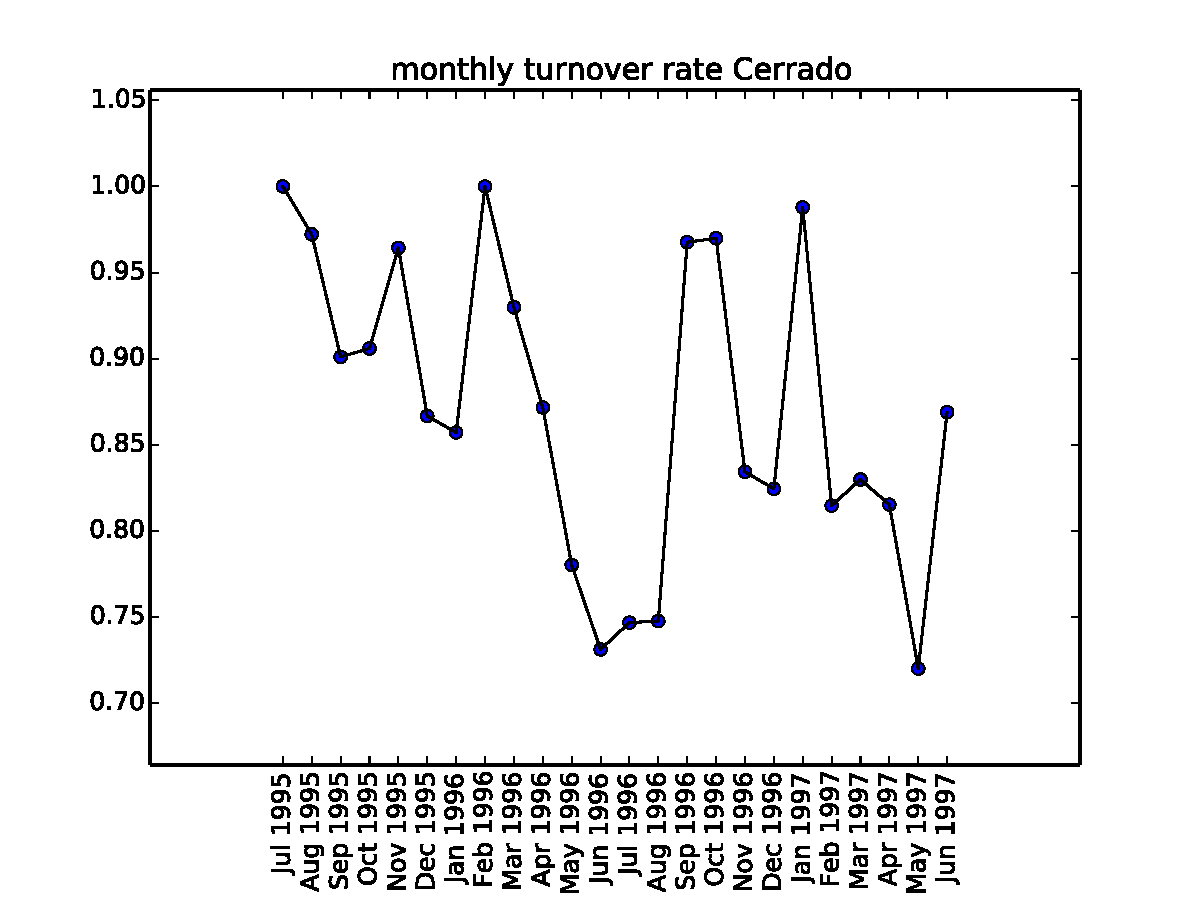
\includegraphics[width=0.8\linewidth]{monthlyCerrado.pdf}
    \footnotesize Representative set of ecosystem flux responses to temperature for different sites from tropical and temperate regions. Y axis show respiration in log scale. 
    
    %If you include your own results (nice if available but not necessary given the early stage of the project) make sure data clearly explained
    
  }
\end{columns}


%%%%%%%%%%%%%%%%%%%%%%%%%%%%%%%%%%%%%%%%%%%%%%%%%%%%%%%%%%%%%%%%%%%%%%%%
\begin{columns}

  \column{0.5}
  \block{\Large \hspace{17pt}Conclusions and Future Research}{ 
  \normalsize	

    \begin{itemize}[itemsep=10pt,topsep=0pt,parsep=0pt,partopsep=0pt, leftmargin=*]
    \item At the intra-specific level, $E_a$ and $T_{peak}$ for $R$ are usually higher than for $P$.
    \item $T_{peak}$’s are usually much higher than the “characteristic” adaptive environment of the organism, so the full unimodal thermal response doesn't matter for mapping individual TPCs to ecosystem-level fluxes.
    \end{itemize}      
%Conclusions that can be drawn and future directions
}
  %%%%%%%%%%%%%%%%%%%%%%%%%%%%%%%%%%%%%%%%%%%%%%%%%%%%%%%%%%%%%%%%%%%%%%%%
  \column{0.5}
  \block{\Large \hspace{17pt}Possible challenges}{
    \normalsize
    \begin{itemize}[itemsep=10pt,topsep=0pt,parsep=0pt,partopsep=0pt, leftmargin=*]
    \item What role might acclimation of intraspecific TPCs play on the ecosystem response?
    \item What is an appropriate distribution for species-level biomass abundances $x_i$?
    \item  Which is the effect of non-linear interactions between species? 
    \end{itemize}    
    %Discussion of research strategy (identification of potential problems and how these will be overcome)

  
}
  
\end{columns}

%%%%%%%%%%%%%%%%%%%%%%%%%%%%%%%%%%%%%%%%%%%%%%%%%%%%%%%%%%%%%%%%%%%%%%%%%%%%%%%%%%%%%%%%%%%%%%%%%%%%%%%%%%%%%%%%%%

\block[bodyverticalshift=-8mm]{}{
  \footnotesize   
  \begin{itemize}[itemsep=10pt,topsep=0pt,parsep=0pt,partopsep=0pt, leftmargin=*]
  \item Enquist, B. J., Economo, E. P., Huxman, T. E., Allen, A. P., Ignace, D. D. and Gillooly, J. F. 2003. Scaling metabolism from organisms to ecosystems. – Nature 423(6940): 639–42.
  \item Savage, V. M. 2004. Improved approximations to scaling relationships for species, populations, and ecosystems across latitudinal and elevational gradients. – J. Theor. Biol. 227(4): 525–534.
  \item Yvon-Durocher, G. and Allen, A. P. 2012. Linking community size structure and ecosystem functioning using metabolic theory. – Philos. Trans. R. Soc. Lond. B. Biol. Sci. 367(1605): 2998–3007.
  \item Yvon-Durocher, et al. 2012. Reconciling the temperature dependence of respiration across timescales and ecosystem types. – Nature 487(7408): 472–6.
  \end{itemize}~\\
  \textit{Acknowledge: This work used eddy covariance data acquired by the FLUXNET community (http://fluxnet.fluxdata.org).}
}


\end{document}
